\section{Testing}
Le testing a été une partie cruciale de notre projet de morphing. Assurer la fiabilité et la précision des algorithmes que nous avons développés nécessitait une approche rigoureuse et méthodique du test. Nous avons mené une série de tests approfondis pour vérifier la robustesse de notre code et garantir que chaque composant fonctionnait comme prévu.
\paragraph{Approche et Méthodologie} Pour tester efficacement notre projet, nous avons adopté une approche en plusieurs étapes :
\begin{itemize}
    \item Tests Unitaires : Nous avons testé chaque fonction individuelle pour s'assurer qu'elle renvoyait les résultats attendus pour un ensemble donné d'entrées.
    \item Tests d'Intégration : Nous avons vérifié que les différentes classes interagissaient correctement lorsqu'elles étaient combinées.
    \item Tests de Régression : Nous avons effectué des tests de régression pour s'assurer que les nouvelles modifications n'altéraient pas le comportement existant de l'application.
    \item Validation Visuelle : Nous avons utilisé des tests visuels pour valider les résultats
\end{itemize}Tests Unitaires :

\paragraph{Remarque.} Les classes des tests peuvent être trouvées en annexe.


\begin{figure}[h!]
    \centering
    \begin{subfigure}{0.45\textwidth}
        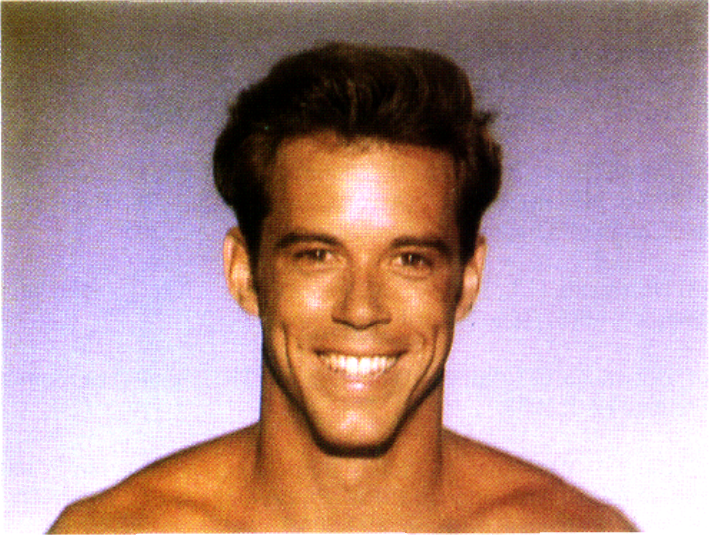
\includegraphics[width=\textwidth]{img/testvisuel/frame0.png}
        \caption{Sous-figure 1}
    \end{subfigure}
    \hfill
    \begin{subfigure}{0.45\textwidth}
        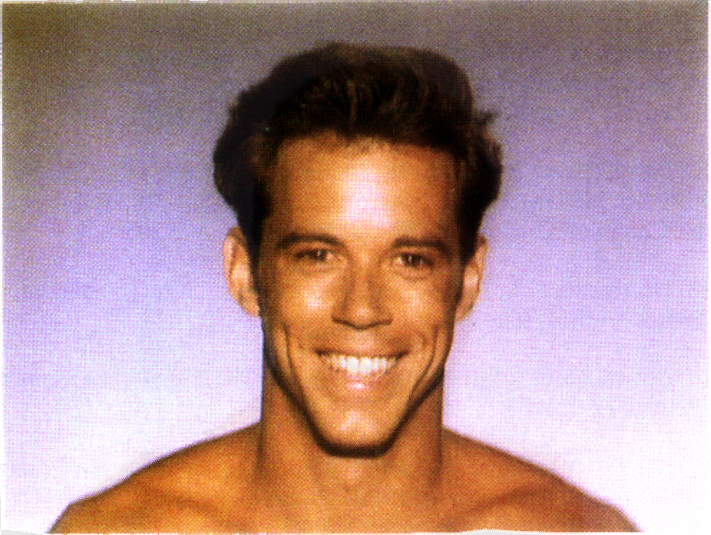
\includegraphics[width=\textwidth]{img/testvisuel/frame1.png}
        \caption{Sous-figure 2}
    \end{subfigure}
    
    \begin{subfigure}{0.45\textwidth}
        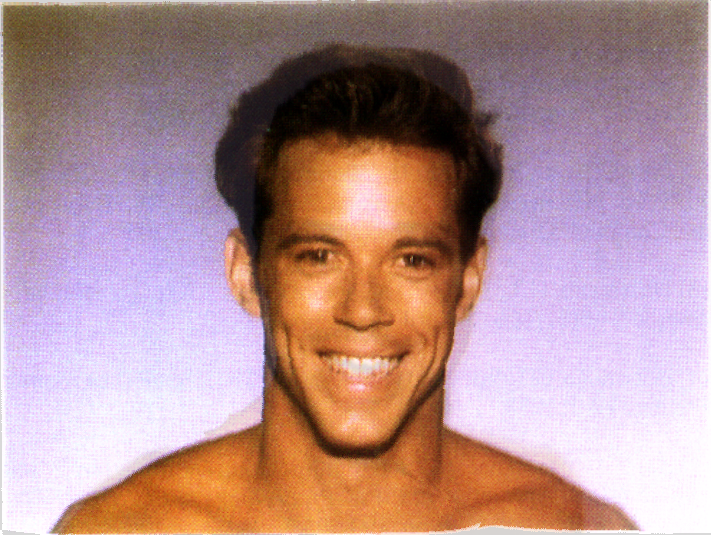
\includegraphics[width=\textwidth]{img/testvisuel/frame2.png}
        \caption{Sous-figure 3}
    \end{subfigure}
    \hfill
    \begin{subfigure}{0.45\textwidth}
        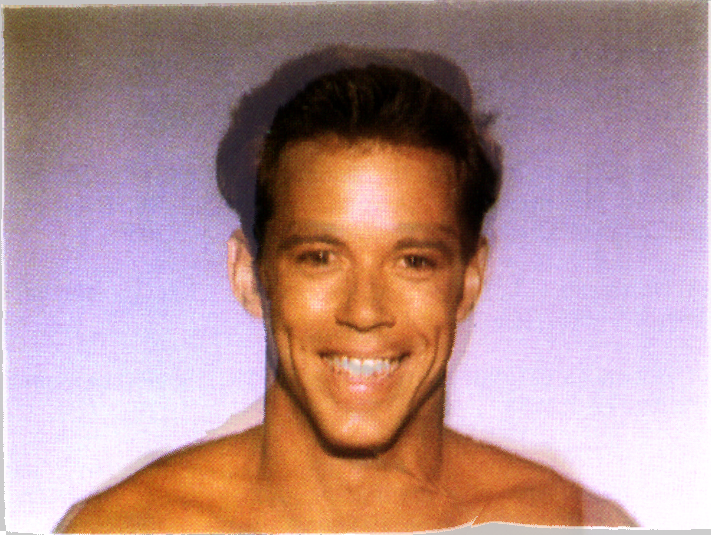
\includegraphics[width=\textwidth]{img/testvisuel/frame3.png}
        \caption{Sous-figure 4}
    \end{subfigure}
\end{figure}

\begin{figure}[h!]
    \begin{subfigure}{0.45\textwidth}
        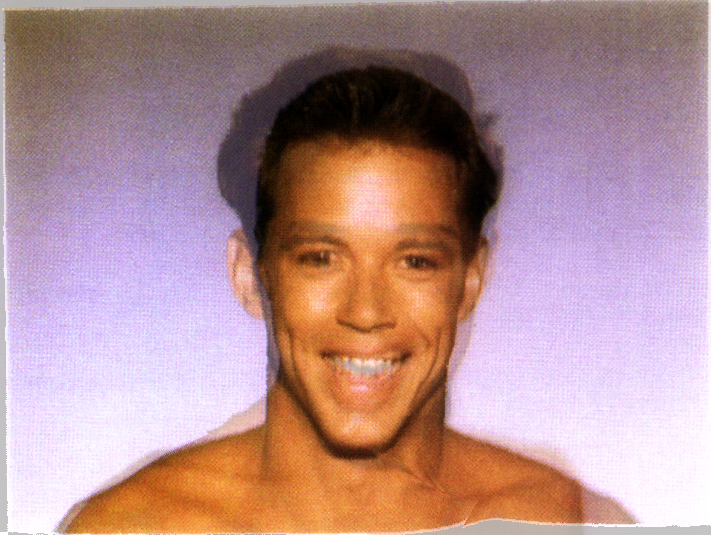
\includegraphics[width=\textwidth]{img/testvisuel/frame4.png}
        \caption{Sous-figure 5}
    \end{subfigure}
    \hfill
    \begin{subfigure}{0.45\textwidth}
        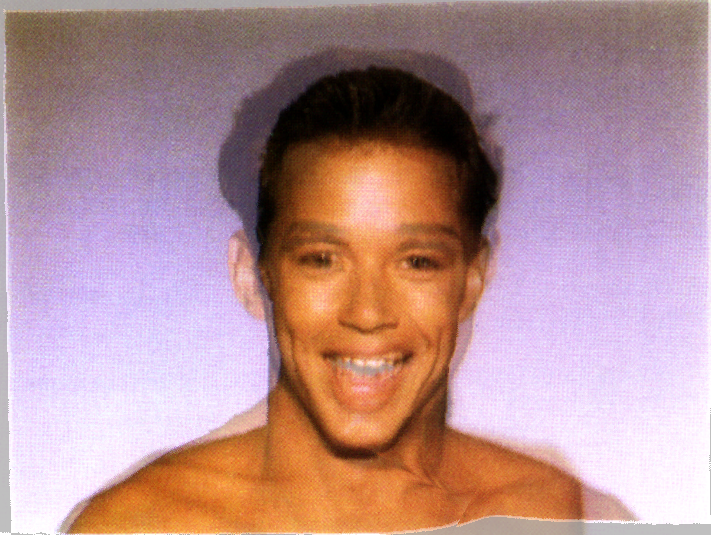
\includegraphics[width=\textwidth]{img/testvisuel/frame5.png}
        \caption{Sous-figure 6}
    \end{subfigure}
    
    \begin{subfigure}{0.45\textwidth}
        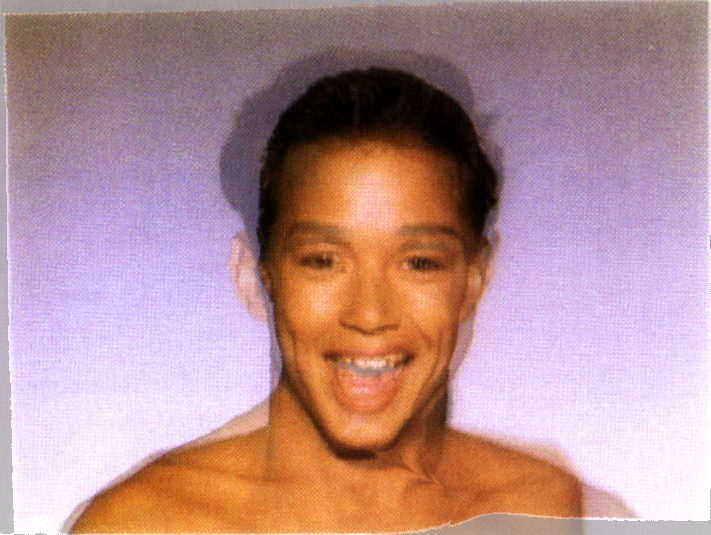
\includegraphics[width=\textwidth]{img/testvisuel/frame6.png}
        \caption{Sous-figure 7}
    \end{subfigure}
    \hfill
    \begin{subfigure}{0.45\textwidth}
        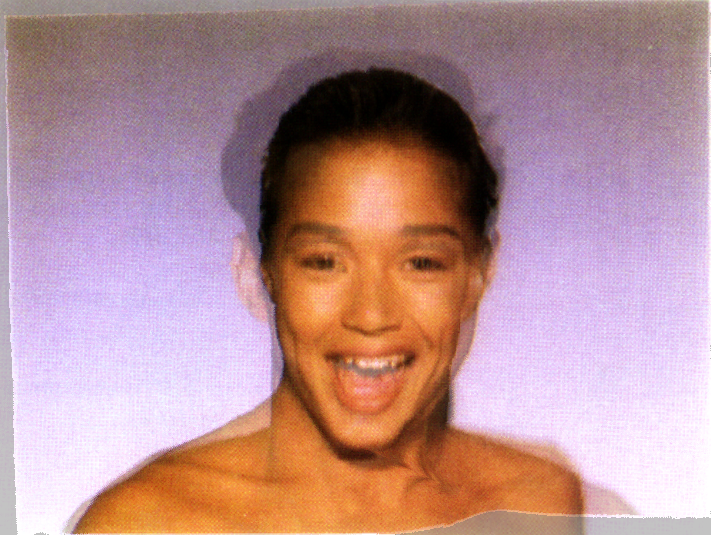
\includegraphics[width=\textwidth]{img/testvisuel/frame7.png}
        \caption{Sous-figure 8}
    \end{subfigure}
    
    \begin{subfigure}{0.45\textwidth}
        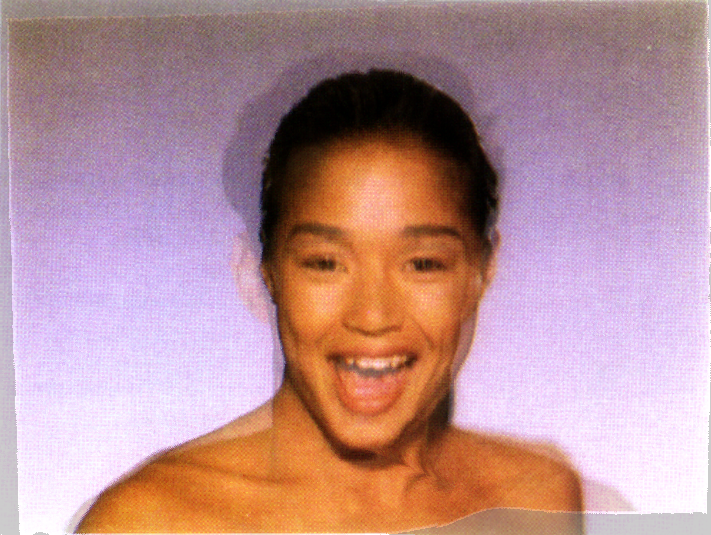
\includegraphics[width=\textwidth]{img/testvisuel/frame8.png}
        \caption{Sous-figure 9}
    \end{subfigure}
    \hfill
    \begin{subfigure}{0.45\textwidth}
        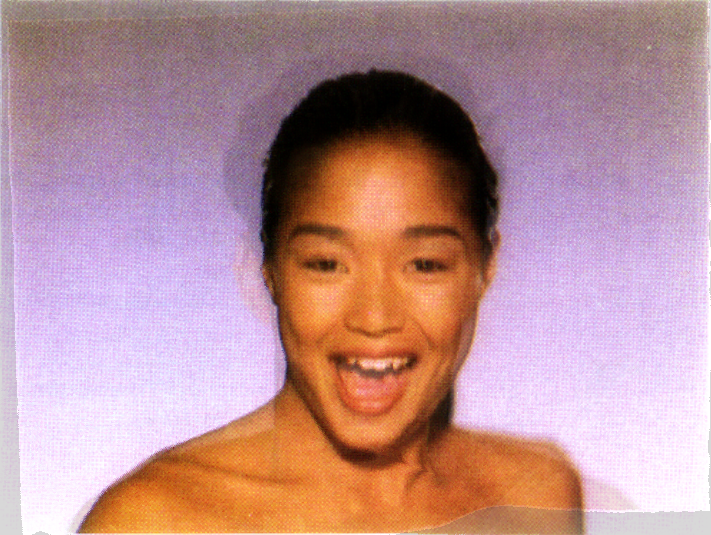
\includegraphics[width=\textwidth]{img/testvisuel/frame9.png}
        \caption{Sous-figure 10}
    \end{subfigure}
    
    \begin{subfigure}{0.45\textwidth}
        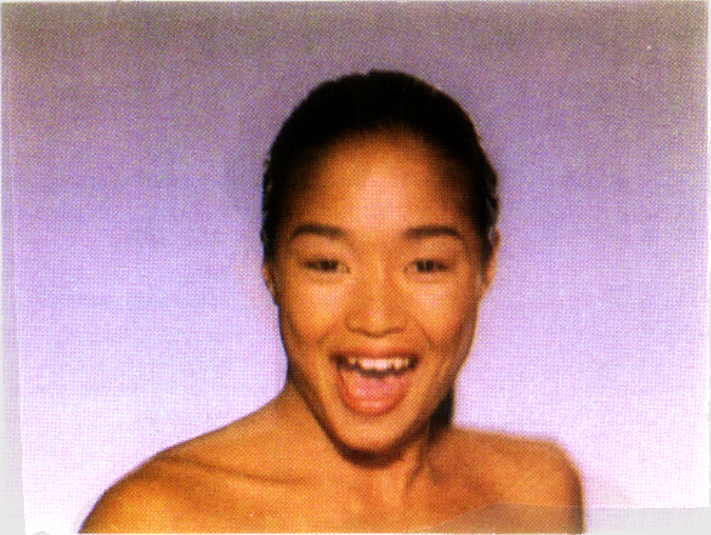
\includegraphics[width=\textwidth]{img/testvisuel/frame10.png}
        \caption{Sous-figure 11}
    \end{subfigure}
    \caption{Résultats des tests visuels}
\end{figure}